% SECTION ON DM HOST MOMENTS
\section{The Host DM and its Moments}\label{sec:moments}
With the cleaned sample, we can characterize the \dmh distribution. We characterize the distribution of \dmh\ via its moments $\langle \dmh \rangle$, as well as higher moments thereof ($\langle \dmh^2 \rangle$, etc.). These moments non-parametrically specify the sightline-to-sightline variation in $\dmh$, and contain information about the spatial distribution of ionized gas relative to that of FRB hosts~\citep{cordes2016radio, reischke2024analytical}. Historically it has been fit to a log-normal distribution with a mean $\muhost$ and width $\sighost$. This parametrization is ubiquitous \citep[e.g.,][]{macquart2020census,james2021z,baptista2024measuring} yet lacks physical justification and has obvious drawbacks. For instance, with the two-parameter log-normal functional form, the RMS scatter in $\dmh$ cannot be decoupled from the heaviness of its tail, i.e. the skew.

To overcome these limitations we directly measure the first four moments (i.e., the mean, width, skew, and excess kurtosis) of the $\dmh$ distribution from the data. Effects such as scattering and propagation through the inclined disks of FRB host galaxies will modify the moments of the $\dmh$ distribution; in the future the locations of FRBs within their host galaxies could potentially be disentangled by their distinct imprints on the moments of the $\dmh$ distribution.

We measure the $\dmh$ moments using our full sample of $z < 0.2$ FRBs as well as three aforementioned subsamples of sources (low-DM, edge-on, and galaxy cluster FRBs). The four moments are defined in Eq.~\ref{eq:mean}-\ref{eq:kurt}. In all cases, each data point is weighted to account for errors in the NE2001 model and an RMS contribution from the cosmic web. In addition, we de-bias the kurtosis estimate (by subtracting 3) such that a Gaussian distribution of \dmh\ values has $\kappa_h = 0$. % , but note that the small redshift range ($z < 0.2$) prevents us from disentangling our fitted parameter $S_h^2$ from 


\begin{align} 
\langle \dmh\rangle &= \dfrac{\sum_i w_i \dmh{}_{,i}}{\sum_i w_i} \label{eq:mean}\\
S_h^2 &= \dfrac{\sum_i w_i (\dmh{}_{,i} - M_h)^2}{\sum_i w_i}\label{eq:std} \\
\Gamma_h &= \dfrac{\sum_i w_i (\dmh{}_{,i} - M_h)^3}{S_h^{3}\sum_i w_i} \label{eq:skew}\\
\kappa_h &= \dfrac{\sum_i w_i (\dmh{}_{,i} - M_h)^4}{S_h^{4}\sum_i w_i} - 3.\label{eq:kurt}
\end{align}

The weights are defined to be $w_i \propto \sigma_i^{-2}$ with
\begin{equation} 
\sigma_i^2 = (0.2\text{DM}_\textrm{NE2001,i})^2 + (10~\text{pc cm}^{-3})^2 + \sigma_\textrm{cosmic}^{2}\label{eq:err_budget}
\end{equation} 
As mentioned in \S~\ref{sec:sample}, this formula accounts for 20\% uncertainties in the Milky Way disk model, a constant uncertainty in the MW halo model, and an RMS scatter in the cosmic dispersion measure originating from haloes as well as the IGM. Measurement uncertainties were estimated by bootstrapping the data with replacement 4000 times. We fix $\sigma_\textrm{cosmic} = 80~\text{pc cm}^{-3}$ in order to be roughly consistent with estimates from~\citet{walker2024dispersion}, but our answers are insensitive to the particular value of $\sigma_\textrm{cosmic}$ used, since it only enters the final estimates through the weighting: fixing $\sigma_\textrm{cosmic} = 0$ shifts the final parameter estimates by at most $5\%$ of their quoted uncertainties. 

Our final parameter estimates for our full sample and various sub-samples are shown in Fig.~\ref{fig:mvsk} and Table~\ref{tab:mvsk}. Measurements from our full sample are precise ($\sim 10\%$). In addition, since they are done with a low-redshift sample of curated sources, they are by construction insensitive to cosmological parameters (Appendix A), robust against changes to the feedback prescription applied to interlopers, or the exact functional form used to parameterize the distribution. They are physically meaningful and apply to isolated, star-forming galaxies between $-22 < M_r < -17$. We also perform measurements for the low-DM, edge-on, and galaxy cluster sub-samples to highlight the effects of those contaminants. 

We can compare our measurements to existing measurements of the host galaxy contribution \citep{james2021z,shin2023inferring,connor2024gas} using analytical expressions which translate the log-normal distribution into non-log space. We compare only the mean, i.e. $\langle \dmh\rangle$ because of each methods' different assumptions. First, the number of bursts cannot be directly translated, since in global fitting analyses, low-redshift bursts constrain the mean host contribution, whereas high-redshift bursts mainly constrain the IGM. In addition, unlocalized and localized FRBs have vastly different constraining power.

The scatter and tail of the distribution cannot be directly compared either, since in those analyses, the RMS host galaxy contribution is divided into host-related and cosmic contributions using an assumed redshift dependence of the latter. In contrast, our measurement makes no assumptions about the redshift dependence but does not allow for the IGM and host contributions to $S_h$ to be separated.

We see no strong trend when binned by host luminosity, nor when dividing the sample by detection experiment. We do find that relative to the clean sample, FRBs in groups, clusters and edge-on host galaxies have much higher values of $\langle \dmh\rangle$ ($> 100$ pc cm$^{-3}$) but similar values of $S_h$ to that of the parent sample. This implies that these systems will bias all cosmological analyses which are sensitive to $\langle\dmh\rangle$.

Third, we find that low-DM selected FRBs have a \dmh\ distribution with much lower mean and standard deviation from the others, implying they should be omitted from population-level cosmological analyses spanning a wide range of redshifts, unless accounted for in a model of the redshift evolution of $\langle\dmh\rangle$. 

Finally, we sub-divide the clean sample into ASKAP/ICS, DSA-110, and CHIME/FRB subsamples (excluding low-DM FRBs for the latter) to check for biases in $\langle\dmh\rangle$ as a function of detection instrument. Each subsample is in agreement at the level of 1$\sigma$ from the others; each subsample is also in agreement with global fitting analyses conducted on samples from each detection experiment, e.g. our sample consisting of bursts detected in the ASKAP/Incoherent Sum Survey (ASKAP/ICS) agrees with the analysis in~\citet{james2021z}, which is dominated by ASKAP/ICS sightlines. Similarly, we see consistency at the 1$\sigma$ level between~\citet{connor2024gas} and our assembled DSA-110 sub-sample. Finally, the CHIME/FRB only sample dramatically improves the constraining power relative to the conclusions of~\citet{shin2023inferring}.

%\begin{figure*}
%    \centering
%    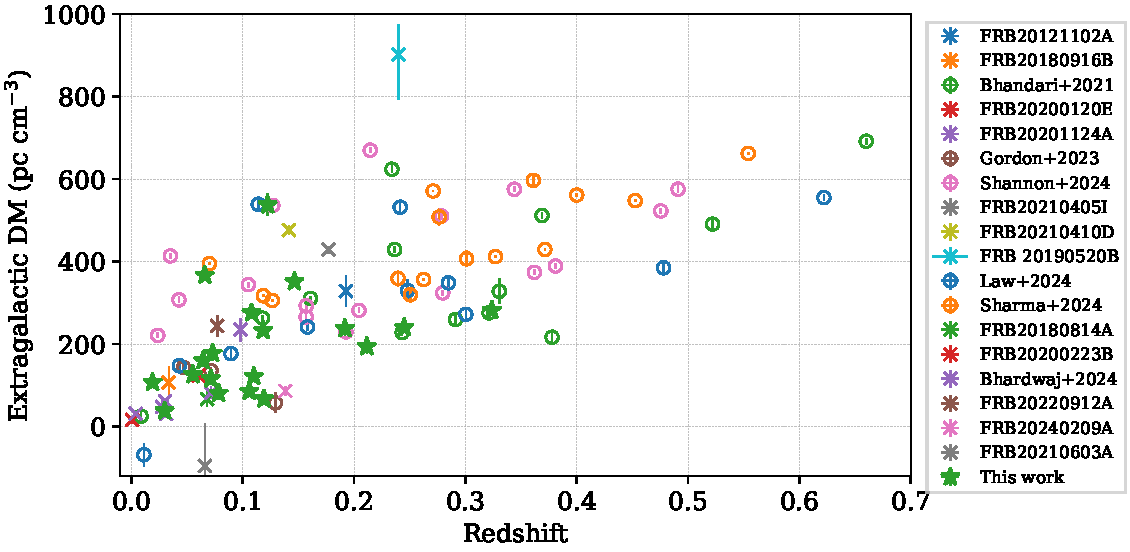
\includegraphics[width=\linewidth]{figures/macquart.pdf}
%    \caption{The redshift-FRB dispersion relation for a selection of host galaxies in the literature shows the complementary redshift coverage of various FRB surveys at the time of this writing. Galaxy redshifts and FRB DM measurements are taken from~\citep{bhandari2022characterizing,gordon2023demographics,law2024deep,sharma2024preferential}. Low-DM selected FRBs from CHIME are taken from ~\citet{bhardwaj2021nearby,michilli2023subarcminute,bhardwaj2024host,Ibik2024host}.}
%    \label{fig:macquart}
%\end{figure*}

The selection effects relevant to this measurement are likely modest. The CHIME/FRB baseband system directly selects against high DM bursts, but this effect is only present when the total DM $> 1000$ pc cm$^{-3}$, and is unlikely to affect our measurement~\citep{collaboration2021first,shin2023inferring}. The CHIME/FRB real-time search pipeline is strongly affected by non-stationary noise, which translates into an lower detection probability for low-flux, highly-scattered bursts. While this could affect the sample of bursts that are detected, we note that bright, highly-scattered bursts are nevertheless detectable~\citep{shin2024investigating}, and that the bursts bright enough to be detected in VLBI should not be strongly subject to this selection effect. We strongly select on host luminosity, because of our localization region, which is usually larger than typical FRB host galaxies. Hence, we caution that our results are only applicable for non-dwarf host galaxies brighter than $M_r < -17$.



\begin{figure*}
    \centering
    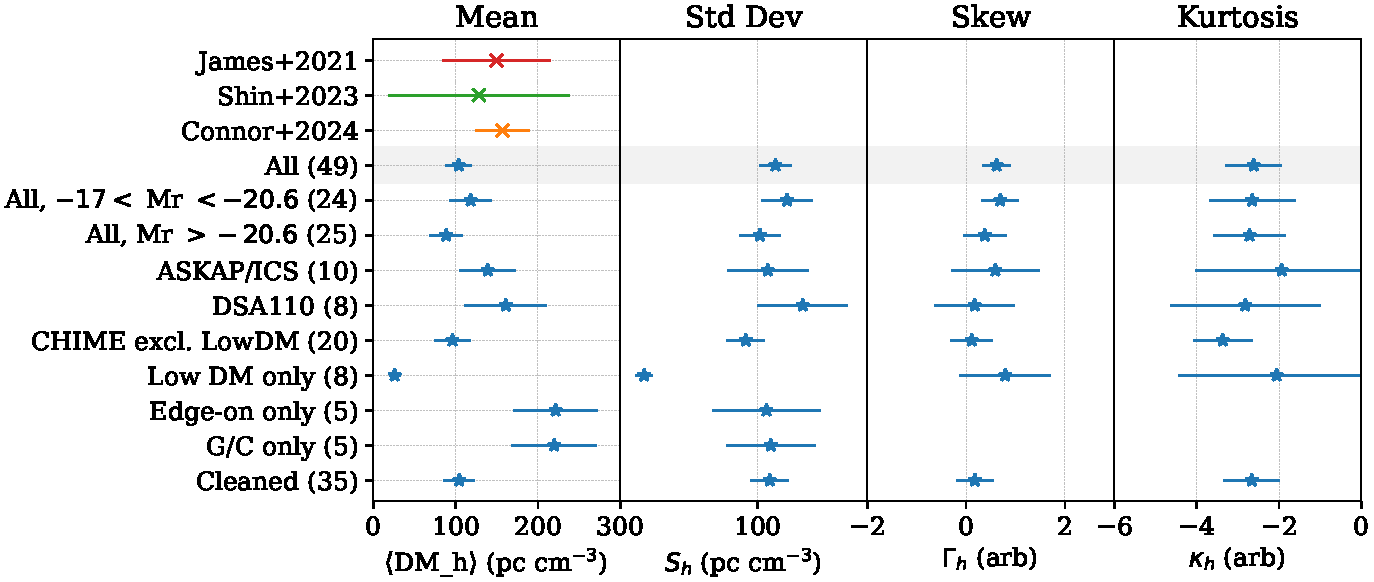
\includegraphics[width=\linewidth]{figures/mvsk.pdf}
    \caption{A graphical representation of Table~\ref{tab:mvsk}, which characterizes the distribution of $\dmh$ using its first four moments. The top three rows show the implied values from global fitting analyses where a log-normal distribution of $\dmh$ is assumed. The shaded grey row denotes the measurement of the \dmh\ distribution using our full sample, which represents the most precise and feedback-insensitive measurement to date.}
    \label{fig:mvsk}
\end{figure*}

\begin{table*}
\caption{Low-redshift estimates of $\langle \dmh\rangle$, $S_h$, $\Gamma_h$,$\kappa_h$ for different subsamples as described in the text. For our measurements, we denote the number of bursts used in each measurement $(N)$, as well as the mean, and standard deviation of the \dmh\ distribution measured in pc cm$^{-3}$, while the skew and excess kurtosis are dimensionless (see text for definitions).}
\begin{tabular}{llllll}
\toprule
 & N & Mean ($\langle\textrm{DM}_h \rangle$) & Std Dev ($S_h$) & Skew ($\Gamma_h$) & Kurtosis ($\kappa_h$) \\
Subsample &  &  &  &  &  \\
\midrule
James+2021 & - & $150 \pm 66$ & $85 \pm 48$ & $1.9 \pm 0.7$ & $7.0 \pm 6.1$ \\
Shin+2023 & - & $128 \pm 110$ & $148 \pm 208$ & - & - \\
Connor+2024 & - & $157 \pm 33$ & $95 \pm 42$ & $2.0 \pm 0.8$ & $8.2 \pm 8.1$ \\
All  & $51$ & $109 \pm 17$ & $115 \pm 12$ & $0.8 \pm 0.3$ & $-2.5 \pm 0.7$ \\
All, $-20.2 < M_r$  & $12$ & $117 \pm 26$ & $87 \pm 18$ & $0.2 \pm 0.7$ & $-2.9 \pm 1.3$ \\
All, $-20.2 > M_r > -21.3$  & $12$ & $117 \pm 26$ & $87 \pm 18$ & $0.2 \pm 0.7$ & $-2.9 \pm 1.3$ \\
All, $M_r < -21.3$  & $11$ & $89 \pm 43$ & $142 \pm 32$ & $0.7 \pm 0.7$ & $-2.5 \pm 1.8$ \\
ASKAP/ICS  & $10$ & $139 \pm 34$ & $107 \pm 29$ & $0.6 \pm 0.9$ & $-1.9 \pm 2.1$ \\
DSA110  & $8$ & $161 \pm 50$ & $133 \pm 33$ & $0.2 \pm 0.8$ & $-2.8 \pm 1.8$ \\
CHIME excl. LowDM  & $22$ & $109 \pm 22$ & $101 \pm 18$ & $0.8 \pm 0.5$ & $-2.3 \pm 1.4$ \\
Low DM only  & $8$ & $26 \pm 7$ & $17 \pm 6$ & $0.8 \pm 0.9$ & $-2.1 \pm 2.4$ \\
Edge-on only  & $5$ & $225 \pm 47$ & $99 \pm 35$ & - & - \\
G/C only  & $5$ & $216 \pm 53$ & $112 \pm 33$ & - & - \\
Cleaned  & $37$ & $111 \pm 19$ & $113 \pm 15$ & $0.5 \pm 0.3$ & $-2.5 \pm 0.7$ \\
\bottomrule
\end{tabular}

\label{tab:mvsk}
\end{table*}